
\section{Prueba 2}


\subsection{Red de inferencia}
\begin{center}
	\tikzstyle{regla}= [rectangle,draw,black,fill=blue!15]
	\tikzstyle{hecho}= [rectangle,draw,black,fill=black!15]
	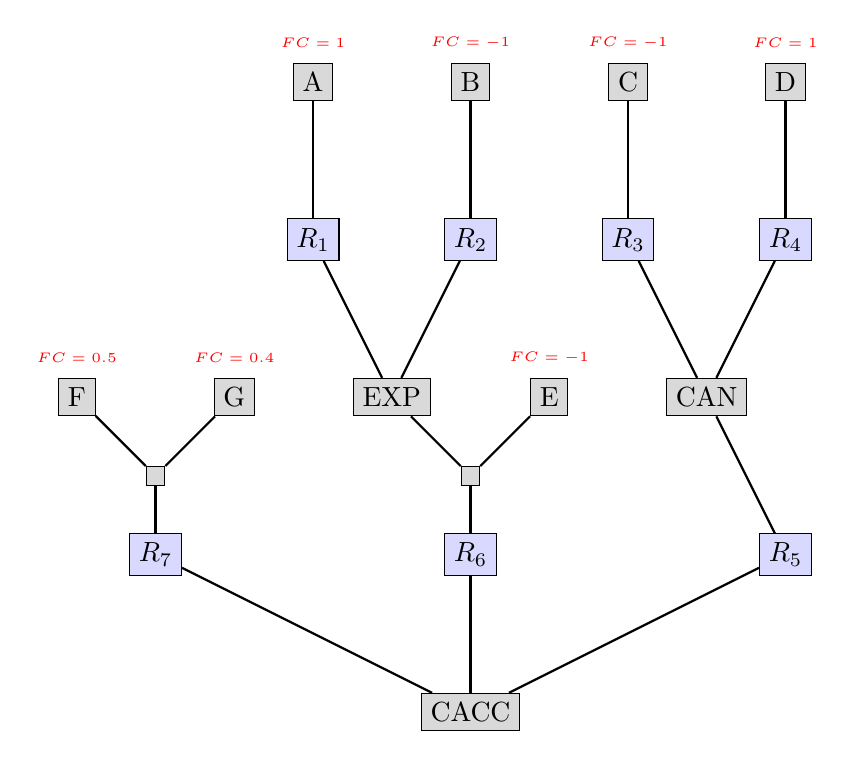
\begin{tikzpicture}
		\node (a) at (3,5) [hecho] {A};
		\node at (3,5.5) {\color{red}{\tiny{$FC=1$}}};

		\node (b) at (5,5) [hecho] {B};
		\node at (5,5.5) {\color{red}{\tiny{$FC=-1$}}};

		\node (c) at (7,5) [hecho] {C};
		\node at (7,5.5) {\color{red}{\tiny{$FC=-1$}}};

		\node (d) at (9,5)[hecho] {D};
		\node at (9,5.5) {\color{red}{\tiny{$FC=1$}}};

		\node (e) at (6,1)[hecho] {E};
		\node at (6,1.5) {\color{red}{\tiny{$FC=-1$}}};

		\node (f) at (0,1)[hecho] {F};
		\node at (0,1.5) {\color{red}{\tiny{$FC=0.5$}}};

		\node (f/g) at (1,0)[hecho] {};
		\node (g) at (2,1)[hecho] {G};
		\node at (2,1.5) {\color{red}{\tiny{$FC=0.4$}}};

		\node (exp) at (4,1)[hecho] {EXP};
		\node (exp/e) at (5,0)[hecho] {};
		
		\node (can) at (8,1)[hecho] {CAN};
		\node (cacc) at (5,-3)[hecho] {CACC};

		\node (r1) at (3,3) [regla] {$R_{1}$};
		\node (r2) at (5,3) [regla] {$R_{2}$};
		\node (r3) at (7,3) [regla] {$R_{3}$};
		\node (r4) at (9,3) [regla] {$R_{4}$};
		\node (r5) at (9,-1) [regla] {$R_{5}$};
		\node (r6) at (5,-1) [regla] {$R_{6}$};
		\node (r7) at (1,-1) [regla] {$R_{7}$};

		\path[black,thick] (a) edge[] node {} (r1);
		\path[black,thick] (b) edge[] node {} (r2);
		\path[black,thick] (c) edge[] node {} (r3);
		\path[black,thick] (d) edge[] node {} (r4);
		\path[black,thick] (f) edge[] node {} (f/g);
		\path[black,thick] (g) edge[] node {} (f/g);
		\path[black,thick] (f/g) edge[] node {} (r7);
		\path[black,thick] (r1) edge[] node {} (exp);
		\path[black,thick] (r2) edge[] node {} (exp);
		\path[black,thick] (r7) edge[] node {} (cacc);
		\path[black,thick] (r6) edge[] node {} (cacc);
		\path[black,thick] (can) edge[] node {} (r5);
		\path[black,thick] (r3) edge[] node {} (can);
		\path[black,thick] (r4) edge[] node {} (can);
		\path[black,thick] (r5) edge[] node {} (cacc);

		\path[black,thick] (exp) edge[] node {} (exp/e);
		\path[black,thick] (e) edge[] node {} (exp/e);
		\path[black,thick] (exp/e) edge[] node {} (r6);
		
		%\draw[->] (b) -- (a);
		\end{tikzpicture}
\end{center}


\subsection{Objetivo obtenido por SBR-FC}

\subsection{Cuestión}
\begin{ejer}
	\textbf{Prueba 2.} En un momento determinado se tiene la siguiente información sobre los hechos:\\
	Se está cumpliendo \texttt{A} con grado 0.6, \texttt{B} con grado 0.4, \texttt{D} con grado 0.9, 
	\texttt{E} con grado 0.7, \texttt{F} con grado 0.8 y \texttt{G} no se está cumpliendo con grado 0.3. \\
	Con esta información, ¿con qué grado se cumple \texttt{I}?
\end{ejer}